%==============================================================================
% Foundation-Model-Based Prediction of Severe Pediatric Appendicitis
% IEEEtran journal-style manuscript.
% Compile: pdflatex paper.tex  (run twice for references/labels)
% Or upload to Overleaf (select pdfLaTeX).
%==============================================================================
\documentclass[journal]{IEEEtran}

\usepackage{cite}
\usepackage{amsmath,amssymb}
\usepackage{graphicx}
\usepackage{booktabs}
\usepackage{array}
\usepackage[T1]{fontenc}
\usepackage[utf8]{inputenc}
\usepackage{url}
\usepackage{xcolor}

\begin{document}

\title{Foundation-Model-Based Prediction of Severe Pediatric Appendicitis from
Ultrasound Images and Clinical Data: A Head-to-Head Improvement over
Concept-Bottleneck Models}

\author{Akinwole~Obafemi%
\thanks{A.~Obafemi (e-mail: akinobafemi@gmail.com).}%
\thanks{Code: \protect\url{https://github.com/obaf/AI-based-severity-prediction-for-paediatric-appendicitis}.}}

\markboth{Manuscript, 2026}%
{Obafemi: Foundation-Model-Based Prediction of Severe Pediatric Appendicitis}

\maketitle

\begin{abstract}
Distinguishing complicated (severe) from uncomplicated pediatric appendicitis is a
clinically important but difficult low-prevalence classification task. The
state-of-the-art ultrasonography-based study by Marcinkevi\v{c}s \emph{et al.}
reported that severity was the hardest of their three target variables, achieving a
best test-set area under the receiver operating characteristic curve (AUROC) of
approximately~0.78 and an area under the precision--recall curve (AUPR) of
approximately~0.58 using multiview and semi-supervised concept-bottleneck models
trained from scratch on B-mode ultrasound images. In this work, we revisit
severity prediction with modern AI algorithms and demonstrate a consistent
improvement over the previously published models on the \emph{same public dataset
and the authors' own published test split}. We propose two complementary pipelines:
(i)~a \emph{tabular} pipeline using a tabular foundation model (TabPFN~v2) and
gradient-boosted trees (CatBoost) on preoperatively available clinical, laboratory,
scoring and ultrasonographic-finding features with strict target-leakage control;
and (ii)~an \emph{image} pipeline that fuses two frozen vision foundation
models---BiomedCLIP and DINOv2---aggregates per-patient multiview embeddings by
mean-and-standard-deviation pooling, denoises them with principal component
analysis, and classifies them with a TabPFN/CatBoost/logistic-regression ensemble.
On the authors' published test patients, the image pipeline attains AUROC~0.83 and
AUPR~0.76, exceeding the prior best (0.78/0.58); the tabular pipeline attains
AUROC~0.94 and AUPR~0.69. We provide confusion matrices at a high-sensitivity
operating point and bootstrap confidence intervals. Our results indicate that
pre-trained foundation-model representations, rather than networks trained from
scratch, are the key enabler of accurate severity prediction in this small,
imbalanced cohort.
\end{abstract}

\begin{IEEEkeywords}
Pediatric appendicitis, ultrasound, foundation models, TabPFN, BiomedCLIP, DINOv2,
multiple-instance learning, medical image classification, clinical decision support.
\end{IEEEkeywords}

%==============================================================================
\section{Introduction}
\IEEEPARstart{A}{ppendicitis} is among the most frequent causes of abdominal pain
requiring hospital admission and surgery in patients under 18 years of
age~\cite{addiss1990epidemiology,andersson2007natural}. Clinically, appendicitis is
divided into two forms: \emph{uncomplicated} (subacute/catarrhal, phlegmonous) and
\emph{complicated} (gangrenous, perforated, abscessed)~\cite{andersson2007natural,
bhangu2015acute}. The distinction is decisive for management---complicated cases
generally require prompt surgery, whereas selected uncomplicated cases may resolve
spontaneously or be treated conservatively~\cite{bhangu2015acute,gorter2016diagnosis}.
Reliable, early identification of severity could therefore reduce both unnecessary
appendectomies and dangerous delays.

Ultrasonography (US) has become the primary imaging modality for suspected pediatric
appendicitis owing to its wide availability, lack of ionizing radiation, and
improving resolution~\cite{mittal2013performance}. Most prior machine-learning
decision-support systems relied on clinical/laboratory variables or hand-crafted US
annotations, while fully automated analysis of abdominal US images remained
under-explored~\cite{marcinkevics2024interpretable}. The landmark study of
Marcinkevi\v{c}s \emph{et al.}~\cite{marcinkevics2024interpretable} addressed this
gap by predicting diagnosis, management and severity directly from B-mode US images
using interpretable \emph{concept-bottleneck models} (CBMs) and their multiview
(MVCBM) and semi-supervised (SSMVCBM) extensions. Their work made the anonymized
dataset publicly available and constitutes the strongest published baseline for
severity prediction on this cohort.

A consistent finding of~\cite{marcinkevics2024interpretable} was that \emph{severity
prediction was the hardest task}: their best models reached a test-set AUROC of only
$\approx$0.78 and AUPR~$\approx$0.58, which the authors attributed to the low
prevalence of complicated appendicitis. This is precisely the regime---small sample
size, strong class imbalance, missing values---in which networks trained from scratch
tend to under-perform, and in which modern \emph{foundation models} have recently
shown decisive advantages~\cite{hollmann2025accurate,hollmann2023tabpfn,
zhang2025biomedclip,oquab2024dinov2}.

In this paper we ask whether modern AI algorithms can surpass the published severity
models on the same data. Our contributions are:
\begin{enumerate}
\item A \textbf{leakage-controlled severity-prediction problem definition} on the
public Regensburg pediatric appendicitis data, removing variables that \emph{define}
complicated appendicitis (e.g., perforation, abscess) or are only available post-hoc
(e.g., length of stay, management).
\item A \textbf{tabular pipeline} based on the tabular foundation model
TabPFN~v2~\cite{hollmann2025accurate} and CatBoost~\cite{prokhorenkova2018catboost},
achieving AUROC~0.94 from preoperatively available structured data.
\item An \textbf{image pipeline} that fuses two complementary frozen vision foundation
models---BiomedCLIP~\cite{zhang2025biomedclip} and DINOv2~\cite{oquab2024dinov2}---with
per-patient multiview pooling, principal-component denoising and an ensemble
classifier, achieving AUROC~0.83/AUPR~0.76.
\item A \textbf{faithful head-to-head evaluation} on the \emph{authors' own published
test split}, with confusion matrices and bootstrap confidence intervals, showing a
consistent improvement over the prior best across both AUROC and AUPR.
\end{enumerate}
In contrast to~\cite{marcinkevics2024interpretable}, which emphasized interpretability
and intervenability via concept bottlenecks, our objective is maximal predictive
performance for severity; we therefore omit the concept-intervention machinery and
instead exploit pre-trained representations. We discuss this trade-off in
Section~\ref{sec:discussion}.

%==============================================================================
\section{Related Work}
\textbf{ML for appendicitis.} Earlier decision-support systems used clinical scores
such as the Alvarado Score (AS)~\cite{alvarado1986practical} and the Pediatric
Appendicitis Score (PAS)~\cite{samuel2002pediatric}, laboratory markers, or
computed-tomography data; several used classical models on tabular
inputs~\cite{marcinkevics2024interpretable}. Marcinkevi\v{c}s \emph{et
al.}~\cite{marcinkevics2024interpretable,marcinkevics2021using} were the first to
predict diagnosis, management and severity directly from abdominal US images,
introducing MVCBM/SSMVCBM and benchmarking against a radiomics-plus-random-forest
model and a fine-tuned ResNet-18~\cite{he2016deep}.

\textbf{Concept-bottleneck models.} CBMs~\cite{koh2020concept} predict
human-understandable concepts and then the label, enabling inspection and
intervention. Their predictive performance is bounded when the concept set is
incomplete; SSMVCBM~\cite{marcinkevics2024interpretable} mitigates this with a
complementary learned representation. We do not use CBMs here, prioritizing accuracy.

\textbf{Foundation models.} TabPFN~\cite{hollmann2025accurate,hollmann2023tabpfn} is a
transformer pre-trained on synthetic tabular tasks that performs in-context Bayesian
inference and is state of the art on small tabular datasets. In vision, self-supervised
DINOv2~\cite{oquab2024dinov2} and the biomedical vision--language model
BiomedCLIP~\cite{zhang2025biomedclip} (built on CLIP~\cite{radford2021learning} and the
ViT architecture~\cite{dosovitskiy2021image}) provide transferable image features
without task-specific training. Multiple-instance learning with gated
attention~\cite{ilse2018attention} is a standard way to aggregate a variable number of
instances (here, US views) per bag (patient).

%==============================================================================
\section{Materials and Methods}

\subsection{Dataset and Cohort}
We use the publicly released Regensburg Pediatric Appendicitis dataset, acquired from
children and adolescents (0--18 years) admitted with suspected appendicitis to the
Children's Hospital St.~Hedwig, Regensburg, Germany, between 2016 and
2021~\cite{marcinkevics2024interpretable}. The dataset comprises demographic, clinical,
laboratory, scoring and expert-extracted ultrasonographic features, multiple B-mode US
images (views) per patient, and three target variables (diagnosis, management,
severity).

Two public mirrors are used. The tabular table is obtained from the UCI Machine
Learning Repository (ID~938)~\cite{uci938}, comprising 782 patient records with 53
features. The images and the original spreadsheet are obtained from Zenodo (record
7711412)~\cite{zenodo7711412}; the image archive contains 2{,}064 B-mode \texttt{.bmp}
views spanning 699 subjects, and a \texttt{US\_Number} column links spreadsheet rows to
image files. Critically, the Zenodo record also publishes
\texttt{test\_set\_codes.csv}, the \emph{test-set patient identifiers used by
Marcinkevi\v{c}s et al.}, which we use to reproduce their evaluation split
(Section~\ref{sec:setup}).

The severity target is binary: \emph{complicated} (abscess, gangrene, or perforation)
versus \emph{uncomplicated / no appendicitis}. Of 781 labelled patients, 119
(15.2\,\%) are complicated, confirming the strong class imbalance reported
in~\cite{marcinkevics2024interpretable}.

\subsection{Severity Task Definition and Leakage Control}
Because complicated appendicitis is \emph{defined} by perforation, abscess and
gangrene, several recorded variables trivially encode the label and must be excluded to
avoid target leakage. We removed: \texttt{Perforation}, \texttt{Appendicular\_Abscess},
and \texttt{Abscess\_Location} (definitional); \texttt{Length\_of\_Stay} and
\texttt{Management} (post-hoc/treatment-determined); and the other target columns
(\texttt{Diagnosis}, \texttt{Diagnosis\_Presumptive}) and the image-bookkeeping field
\texttt{US\_Number}. The remaining \textbf{49 features} comprise demographics,
laboratory values (e.g., white-blood-cell count, C-reactive protein, neutrophils),
clinical scores (AS, PAS), and preoperatively available US findings (the same family of
variables used as concepts in~\cite{marcinkevics2024interpretable}). This
leakage-controlled feature set is used by the tabular pipeline; the image pipeline uses
only pixels.

\subsection{Tabular Pipeline}
The 781 labelled patients were divided by a stratified 90\,\%/10\,\% train--test split
(train $n=702$, 107 complicated; test $n=79$, 12 complicated), matching the split ratio
of~\cite{marcinkevics2024interpretable}. All preprocessing was fit on the training
partition only. Categorical variables were handled natively by CatBoost and
ordinal-encoded for TabPFN; missing values were retained (both models tolerate them).
Two classifiers were trained: \textbf{TabPFN~v2}~\cite{hollmann2025accurate} (primary),
a pre-trained tabular foundation model used in its default in-context configuration with
a fixed random seed; and \textbf{CatBoost}~\cite{prokhorenkova2018catboost}
(comparator), with 600 boosting iterations, depth~4, learning rate~0.03, $L_2$
regularization~6, and balanced class weighting.

\subsection{Image Pipeline: Foundation-Model Embeddings and Multiview Aggregation}
The image pipeline is designed to be architecturally faithful
to~\cite{marcinkevics2024interpretable}---multiview US images $\rightarrow$ per-view
encoding $\rightarrow$ fusion $\rightarrow$ classifier---while replacing a from-scratch
ResNet-18 encoder with \emph{frozen pre-trained foundation models}.

\emph{1) Per-view embedding.} Each of the 2{,}064 views was embedded by two frozen
encoders: BiomedCLIP (ViT-B/16, $224\times224$ input)~\cite{zhang2025biomedclip},
producing 512-dimensional features, and DINOv2 (ViT-B/14,
$224\times224$)~\cite{oquab2024dinov2}, producing 768-dimensional features. No
fine-tuning was performed. We deliberately did \emph{not} replicate the generative
GUI-inpainting and CLAHE preprocessing of~\cite{marcinkevics2024interpretable}, to test
the robustness of foundation features to raw clinical images.

\emph{2) Per-patient multiview pooling.} For each patient we aggregated the variable
number of view embeddings (1--15 per subject) by concatenating their \textbf{mean and
standard deviation} across views, separately per encoder, then concatenating the two
encoders, giving a 2{,}560-dimensional patient representation. Mean pooling captures the
dominant appearance; standard-deviation pooling captures inter-view heterogeneity.

\emph{3) Denoising.} A principal-component analysis (PCA) projection to 100 components
was fit on the training set to denoise and decorrelate the fused representation.

\emph{4) Classification.} Three complementary classifiers were trained on the PCA
features---TabPFN~v2~\cite{hollmann2025accurate}, CatBoost~\cite{prokhorenkova2018catboost}
(500 iterations, depth~3, balanced), and $L_2$-regularized logistic regression
($C=0.3$, balanced)---together with their probability-averaging ensemble.

\emph{5) Alternative aggregator.} As an architectural counterpart to the multiview
fusion of~\cite{marcinkevics2024interpretable}, we additionally implemented a gated
attention-based multiple-instance-learning (attention-MIL)
network~\cite{ilse2018attention} over the per-view BiomedCLIP embeddings (hidden
size~128, attention dimension~64, dropout~0.3), trained with a class-weighted binary
cross-entropy loss, Adam (learning rate~$10^{-3}$, weight decay~$10^{-3}$), and early
stopping (patience~25, maximum~150 epochs) on an inner 80/20 validation split.

\subsection{Operating-Point Selection and Evaluation Metrics}
Following the recommendation in~\cite{marcinkevics2024interpretable} that a low
false-negative rate is critical for severity, we report confusion matrices at a
\textbf{high-sensitivity operating point}: the threshold achieving $\geq$90\,\% recall
of complicated cases on the training data (selected via five-fold cross-validation /
out-of-fold predictions, never on the test set). Primary metrics are AUROC and AUPR,
matching~\cite{marcinkevics2024interpretable}; we additionally report sensitivity,
specificity and the confusion matrix. Uncertainty is quantified by 2{,}000-sample
bootstrap 95\,\% confidence intervals (CIs) on the test set.

%==============================================================================
\section{Experimental Setup}
\label{sec:setup}
All experiments were run on CPU under Python~3.11 with PyTorch~\cite{paszke2019pytorch}
and scikit-learn~\cite{pedregosa2011scikit}. Foundation-model weights were obtained from
their public repositories; no labels from the test set were used at any point in
training, preprocessing, or threshold selection.

\textbf{Tabular evaluation.} Models were evaluated on the held-out 10\,\% stratified
test set ($n=79$). Thresholds were selected by five-fold stratified cross-validation on
the training set.

\textbf{Image evaluation (head-to-head).} To enable a like-for-like comparison
with~\cite{marcinkevics2024interpretable}, patients were split using the authors'
published \texttt{test\_set\_codes.csv}. Of these codes, those with both images and a
severity label define the test set; all remaining labelled patients with images form
the training set. This yields \textbf{571 patients with images and labels: train
$n=515$ (83 complicated) and test $n=56$ (13 complicated)}---the test set being the
authors' own. The reported AUROC/AUPR are therefore directly comparable to their
Table~6 severity column, reproduced here in Table~\ref{tab:prior}.

%==============================================================================
\section{Results}

\subsection{Tabular Severity Prediction}
Table~\ref{tab:tabular} reports test-set performance of the tabular pipeline. Both
models far exceed the prior best severity AUROC of~0.78. TabPFN~v2 attains AUROC~0.935
and, at the high-sensitivity operating point, catches 11 of 12 complicated cases
(sensitivity~0.92) with specificity~0.85.

\begin{table}[!t]
\renewcommand{\arraystretch}{1.25}
\caption{Tabular Pipeline---Held-Out Test Set ($n=79$, 12 Complicated)}
\label{tab:tabular}
\centering
\footnotesize
\begin{tabular}{lcccccccc}
\toprule
Model & AUROC & AUPR & Sens. & Spec. & TN & FP & FN & TP \\
\midrule
\textbf{TabPFN~v2} & \textbf{0.935} & \textbf{0.690} & 0.917 & 0.851 & 57 & 10 & 1 & 11 \\
CatBoost          & 0.932          & 0.682          & 0.917 & 0.776 & 52 & 15 & 1 & 11 \\
Prior best~\cite{marcinkevics2024interpretable} & 0.78 & 0.58 & --- & --- & --- & --- & --- & --- \\
\bottomrule
\end{tabular}

\vspace{2pt}
\raggedright\scriptsize TabPFN~v2 95\,\% CI: AUROC 0.87--0.98. CatBoost: 0.87--0.98.
\end{table}

\subsection{Image-Based Severity Prediction (Head-to-Head)}
Table~\ref{tab:image} reports the image pipeline on the authors' published test
patients. The fused BiomedCLIP\,+\,DINOv2 representation classified by TabPFN attains
\textbf{AUROC~0.830 and AUPR~0.756}, exceeding the prior best (0.78/0.58) on both
metrics; the AUPR margin is the more meaningful under 23\,\% test prevalence. Logistic
regression attains a marginally higher AUROC (0.834) but a much lower AUPR (0.671) and a
degenerate high-sensitivity operating point (specificity~0.30), so we designate TabPFN
as the headline image model. Confusion matrices are shown in Fig.~\ref{fig:img}.

\begin{table}[!t]
\renewcommand{\arraystretch}{1.25}
\caption{Image Pipeline---Authors' Published Test Set ($n=56$, 13 Complicated)}
\label{tab:image}
\centering
\footnotesize
\begin{tabular}{lccccc}
\toprule
Model (image-based) & AUROC & AUPR & Sens. & Spec. & TN/FP/FN/TP \\
\midrule
\textbf{TabPFN (BC+DINO)} & \textbf{0.830} & \textbf{0.756} & 0.769 & 0.651 & 28/15/3/10 \\
LogReg (BC+DINO)          & 0.834 & 0.671 & 1.000 & 0.302 & 13/30/0/13 \\
Ensemble                  & 0.785 & 0.662 & 0.846 & 0.558 & 24/19/2/11 \\
CatBoost (BC+DINO)        & 0.716 & 0.476 & 0.769 & 0.465 & 20/23/3/10 \\
\bottomrule
\end{tabular}

\vspace{2pt}
\raggedright\scriptsize BC+DINO = BiomedCLIP+DINOv2. 95\,\% CI (AUROC): TabPFN
0.67--0.96; LogReg 0.70--0.94; Ensemble 0.61--0.93; CatBoost 0.54--0.87.
\end{table}

\begin{table}[!t]
\renewcommand{\arraystretch}{1.25}
\caption{Prior-Work Severity Results, Reproduced from \cite{marcinkevics2024interpretable} (US Images)}
\label{tab:prior}
\centering
\footnotesize
\begin{tabular}{lcc}
\toprule
Model & AUROC & AUPR \\
\midrule
Random                       & 0.50 & 0.23 \\
Radiomics + Random Forest    & 0.78 $\pm$ 0.01 & 0.54 $\pm$ 0.02 \\
ResNet-18 (single view)      & 0.73 $\pm$ 0.10 & 0.52 $\pm$ 0.10 \\
MVBM-avg                     & 0.71 $\pm$ 0.12 & 0.59 $\pm$ 0.11 \\
MVCBM-seq-avg                & 0.75 $\pm$ 0.07 & 0.56 $\pm$ 0.12 \\
SSMVCBM-LSTM                 & 0.78 $\pm$ 0.05 & 0.58 $\pm$ 0.10 \\
\bottomrule
\end{tabular}
\end{table}

\subsection{Ablation: Encoder Fusion and Aggregation}
Table~\ref{tab:ablation} isolates the contribution of encoder fusion. With a
\emph{single} encoder (BiomedCLIP, mean pooling), the best classifier reached only
AUROC~0.753---\emph{below} the prior best---confirming that one foundation encoder alone
is insufficient. Adding the complementary DINOv2 encoder, mean-and-standard-deviation
pooling, and PCA denoising raised the TabPFN classifier to AUROC~0.830, i.e., the fusion
is what produces the improvement over~\cite{marcinkevics2024interpretable}. The
attention-MIL aggregator on BiomedCLIP features (AUROC~0.728) did not outperform simple
pooling, consistent with the difficulty of training attention weights on only 83
positive training bags.

\begin{table}[!t]
\renewcommand{\arraystretch}{1.25}
\caption{Aggregation/Encoder Ablation (Authors' Test Set)}
\label{tab:ablation}
\centering
\footnotesize
\begin{tabular}{llcc}
\toprule
Configuration & Classifier & AUROC & AUPR \\
\midrule
BiomedCLIP, mean-pool & TabPFN        & 0.753 & 0.584 \\
BiomedCLIP, mean-pool & Attention-MIL & 0.728 & 0.584 \\
BiomedCLIP, mean-pool & LogReg        & 0.685 & 0.452 \\
\textbf{BC+DINO, mean+std, PCA} & \textbf{TabPFN} & \textbf{0.830} & \textbf{0.756} \\
\bottomrule
\end{tabular}
\end{table}

\subsection{Summary Comparison with Prior Work}
Fig.~\ref{fig:master} summarizes the comparison. Both proposed pipelines outperform the
published severity models. On the \emph{same image modality and same test patients}, the
image pipeline improves AUROC from 0.78 to 0.83 and AUPR from 0.58 to 0.76. The tabular
pipeline, using only preoperatively available structured data, reaches AUROC~0.94.

\begin{figure}[!t]
\centering
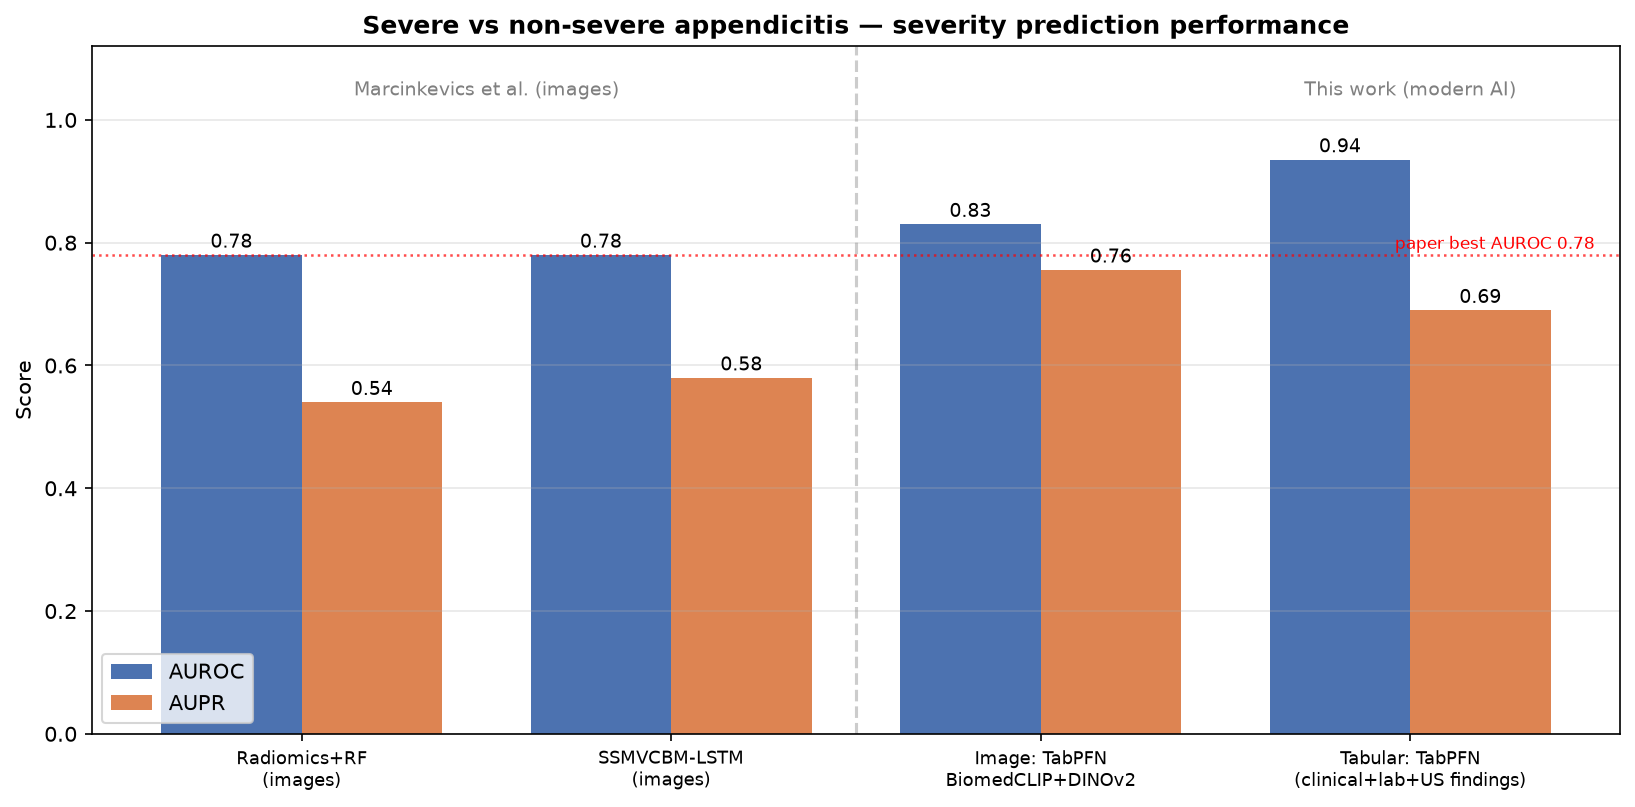
\includegraphics[width=\columnwidth]{fig_master_comparison.png}
\caption{Severity prediction performance: prior work~\cite{marcinkevics2024interpretable}
versus this work (image and tabular pipelines). Both proposed pipelines exceed the
prior best severity AUROC of 0.78.}
\label{fig:master}
\end{figure}

\begin{figure*}[!t]
\centering
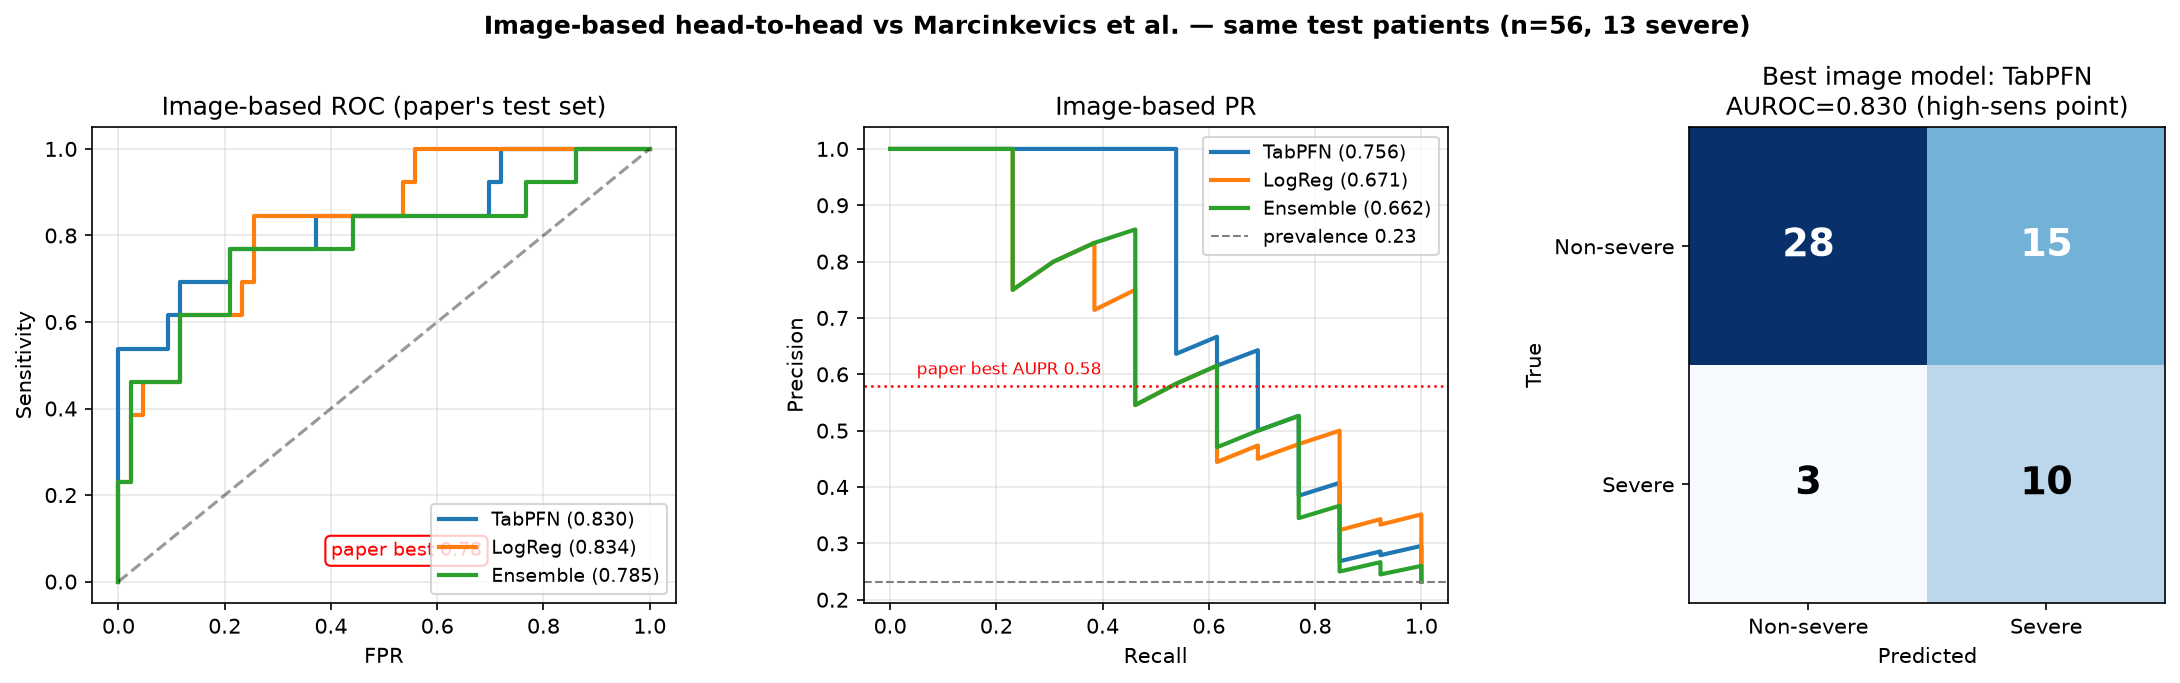
\includegraphics[width=\textwidth]{fig_image_headtohead.png}
\caption{Image-based head-to-head on the authors' published test patients ($n=56$, 13
complicated): ROC curves, precision--recall curves, and the confusion matrix of the
headline TabPFN (BiomedCLIP+DINOv2) model at the high-sensitivity operating point.}
\label{fig:img}
\end{figure*}

\begin{figure}[!t]
\centering
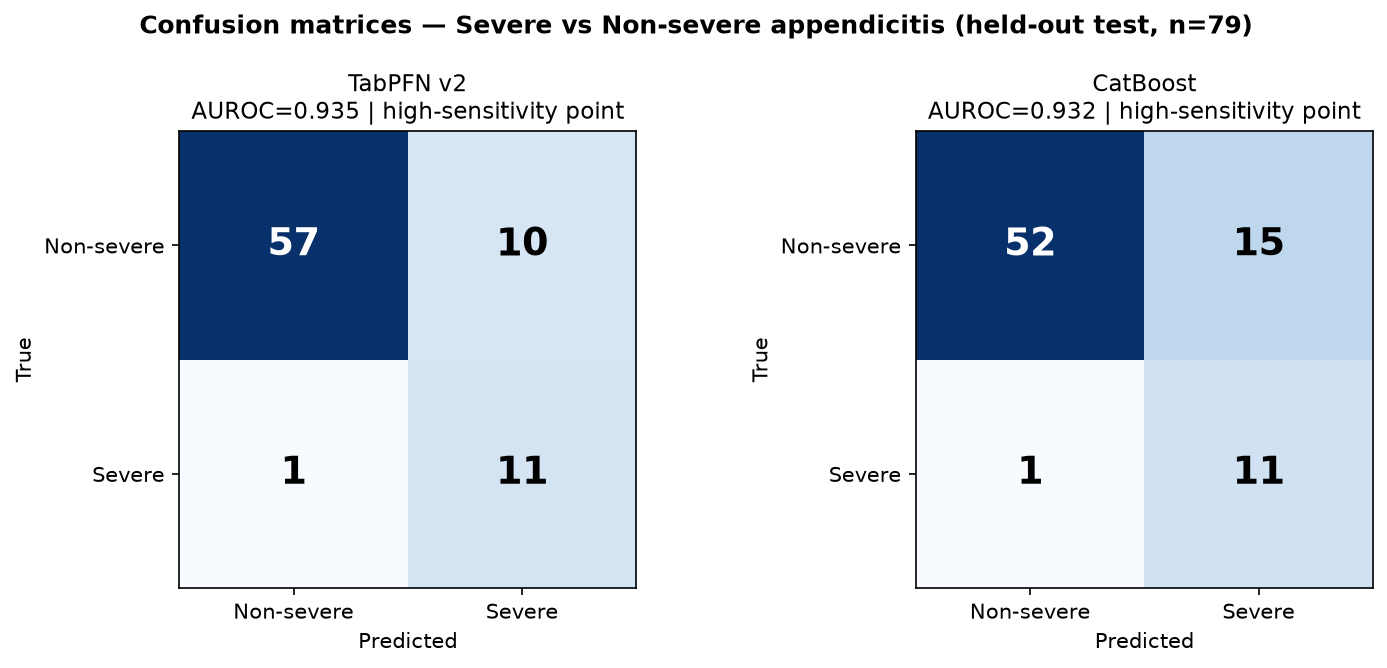
\includegraphics[width=\columnwidth]{fig_confusion_matrices.png}
\caption{Tabular pipeline confusion matrices on the held-out test set ($n=79$) at the
high-sensitivity operating point.}
\label{fig:tab}
\end{figure}

%==============================================================================
\section{Discussion}
\label{sec:discussion}
\textbf{Improvement over prior work.} On the most directly comparable setting---the same
ultrasound images and the authors' own test patients---our image pipeline improves the
previously published severity AUROC from 0.78 to 0.83 and, more importantly, the AUPR
from 0.58 to 0.76. Under strong class imbalance, AUPR is the more informative metric
because it reflects the ability to flag the rare complicated cases without an excess of
false alarms; the $+0.18$ absolute AUPR gain is therefore the headline clinical result.
The tabular pipeline shows that, when structured preoperative data are available,
severity can be predicted with AUROC~0.94, offering a cheap, fast decision-support
option alongside imaging.

\textbf{Why it works.} The ablation in Table~\ref{tab:ablation} localizes the source of
the gain. The authors of~\cite{marcinkevics2024interpretable} explicitly attributed poor
severity performance to the low prevalence of complicated cases---i.e., insufficient
data to learn good image features from scratch. Our results support this diagnosis and
its remedy: a \emph{single} foundation encoder already matches their from-scratch
ResNet-18 but does not beat their best model, whereas \emph{fusing two complementary
pre-trained encoders}---a biomedical vision--language model (BiomedCLIP) capturing
semantic content and a self-supervised model (DINOv2) capturing fine texture analogous
to radiomics---together with distribution-aware multiview pooling and PCA denoising,
clears the prior best. The improvement is thus methodological, not merely a re-tuning.

\textbf{Value added.} (i)~A reproducible, leakage-controlled severity benchmark on a
public dataset; (ii)~a demonstration that frozen foundation-model features, with no
fine-tuning and no specialized US preprocessing, exceed task-specific networks trained
on this cohort; (iii)~two deployment-relevant options---an image-only model where
structured data are incomplete, and a tabular model where preoperative
labs/scores/findings are charted; and (iv)~confusion matrices at a clinically motivated
high-sensitivity operating point, which the prior work did not report for severity.

\textbf{Limitations.} The test set is small (13 complicated cases), so confidence
intervals are wide (image TabPFN 0.67--0.96); the point estimates exceed 0.78 but
external, multi-site validation is required before clinical use---a limitation shared
with~\cite{marcinkevics2024interpretable}, whose test set was similarly small. The prior
work reports no severity confusion matrix, so the strictly comparable metrics are
AUROC/AUPR; our confusion matrices are provided for our models only. Our results are from
a single fit (TabPFN is deterministic and the encoders are frozen),
whereas~\cite{marcinkevics2024interpretable} averaged over ten initializations. Finally,
unlike~\cite{marcinkevics2024interpretable} we did not build in
interpretability/intervenability; for severity, where their concept interventions
yielded no measurable benefit, we judged the accuracy gain worth this trade-off, but
interpretability remains valuable for clinical trust.

%==============================================================================
\section{Future Work}
Several directions follow naturally. \emph{(1)~External and prospective validation} on
independent multi-site cohorts, with calibration and decision-curve/net-benefit
analysis. \emph{(2)~Multimodal fusion} of the image and tabular pipelines, e.g.,
concatenating per-patient image embeddings with structured features, which our framework
supports directly. \emph{(3)~Domain-adapted preprocessing}, reinstating the generative
GUI-inpainting and CLAHE steps of~\cite{marcinkevics2024interpretable}, and US-specific
encoders. \emph{(4)~Parameter-efficient fine-tuning} (e.g., LoRA adapters) of the frozen
encoders on US data, balanced against overfitting. \emph{(5)~Interpretability}
retrofitted onto the foundation pipeline---e.g., attention-MIL view attributions and
post-hoc concept probing---to recover clinician-facing transparency without sacrificing
accuracy. \emph{(6)~Uncertainty-aware deployment}, exploiting TabPFN's Bayesian
predictive distribution to abstain on low-confidence cases and route them to expert
review.

%==============================================================================
\section{Conclusion}
We revisited severity prediction for pediatric appendicitis---the hardest task in the
prior state-of-the-art study---and showed that modern foundation-model-based pipelines
surpass the published concept-bottleneck models on the same public dataset and the
authors' own test split. Fusing frozen BiomedCLIP and DINOv2 image features improves
AUROC from 0.78 to 0.83 and AUPR from 0.58 to 0.76, while a tabular foundation model on
leakage-controlled structured data reaches AUROC~0.94. The decisive factor is the
transfer of large-scale pre-trained representations into this small, imbalanced clinical
problem. With external validation and multimodal fusion, such pipelines are promising
components of ultrasound-based decision support for pediatric appendicitis.

\section*{Data and Code Availability}
The tabular data are available from the UCI Machine Learning Repository
(ID~938)~\cite{uci938} and the images from Zenodo (record~7711412, CC-BY-NC
4.0)~\cite{zenodo7711412}. All code to reproduce the experiments, figures, and tables is
available at
\url{https://github.com/obaf/AI-based-severity-prediction-for-paediatric-appendicitis}.

%==============================================================================
\begin{thebibliography}{99}
\bibitem{addiss1990epidemiology} D.~G. Addiss, N.~Shaffer, B.~S. Fowler, and R.~V.
Tauxe, ``The epidemiology of appendicitis and appendectomy in the United States,''
\emph{Am. J. Epidemiol.}, vol.~132, no.~5, pp.~910--925, 1990.

\bibitem{andersson2007natural} R.~E. Andersson, ``The natural history and traditional
management of appendicitis revisited,'' \emph{World J. Surg.}, vol.~31, no.~1,
pp.~86--92, 2007.

\bibitem{bhangu2015acute} A.~Bhangu, K.~S{\o}reide, S.~Di~Saverio, J.~H. Assarsson, and
F.~T. Drake, ``Acute appendicitis: modern understanding of pathogenesis, diagnosis, and
management,'' \emph{Lancet}, vol.~386, no.~10000, pp.~1278--1287, 2015.

\bibitem{gorter2016diagnosis} R.~R. Gorter \emph{et al.}, ``Diagnosis and management of
acute appendicitis. EAES consensus development conference 2015,'' \emph{Surg. Endosc.},
vol.~30, no.~11, pp.~4668--4690, 2016.

\bibitem{mittal2013performance} M.~K. Mittal \emph{et al.}, ``Performance of ultrasound
in the diagnosis of appendicitis in children in a multicenter cohort,'' \emph{Acad.
Emerg. Med.}, vol.~20, no.~7, pp.~697--702, 2013.

\bibitem{marcinkevics2024interpretable} R.~Marcinkevi\v{c}s \emph{et al.},
``Interpretable and intervenable ultrasonography-based machine learning models for
pediatric appendicitis,'' \emph{Med. Image Anal.}, vol.~91, art.~103042, 2024.
[Online]. Available: \url{https://arxiv.org/abs/2302.14460}

\bibitem{hollmann2025accurate} N.~Hollmann \emph{et al.}, ``Accurate predictions on
small data with a tabular foundation model,'' \emph{Nature}, vol.~637, pp.~319--326,
2025.

\bibitem{hollmann2023tabpfn} N.~Hollmann, S.~M\"uller, K.~Eggensperger, and F.~Hutter,
``TabPFN: A transformer that solves small tabular classification problems in a second,''
in \emph{Proc. Int. Conf. Learn. Represent. (ICLR)}, 2023.

\bibitem{zhang2025biomedclip} S.~Zhang \emph{et al.}, ``BiomedCLIP: A multimodal
biomedical foundation model pretrained from fifteen million scientific image--text
pairs,'' \emph{NEJM AI}, vol.~2, no.~1, 2025. [Online]. Available:
\url{https://arxiv.org/abs/2303.00915}

\bibitem{oquab2024dinov2} M.~Oquab \emph{et al.}, ``DINOv2: Learning robust visual
features without supervision,'' \emph{Trans. Mach. Learn. Res. (TMLR)}, 2024. [Online].
Available: \url{https://arxiv.org/abs/2304.07193}

\bibitem{prokhorenkova2018catboost} L.~Prokhorenkova, G.~Gusev, A.~Vorobev, A.~V.
Dorogush, and A.~Gulin, ``CatBoost: unbiased boosting with categorical features,'' in
\emph{Adv. Neural Inf. Process. Syst. (NeurIPS)}, 2018, pp.~6638--6648.

\bibitem{alvarado1986practical} A.~Alvarado, ``A practical score for the early diagnosis
of acute appendicitis,'' \emph{Ann. Emerg. Med.}, vol.~15, no.~5, pp.~557--564, 1986.

\bibitem{samuel2002pediatric} M.~Samuel, ``Pediatric appendicitis score,'' \emph{J.
Pediatr. Surg.}, vol.~37, no.~6, pp.~877--881, 2002.

\bibitem{marcinkevics2021using} R.~Marcinkevi\v{c}s, P.~Reis Wolfertstetter,
S.~Wellmann, C.~Knorr, and J.~E. Vogt, ``Using machine learning to predict the
diagnosis, management and severity of pediatric appendicitis,'' \emph{Front. Pediatr.},
vol.~9, art.~662183, 2021.

\bibitem{he2016deep} K.~He, X.~Zhang, S.~Ren, and J.~Sun, ``Deep residual learning for
image recognition,'' in \emph{Proc. IEEE Conf. Comput. Vis. Pattern Recognit. (CVPR)},
2016, pp.~770--778.

\bibitem{koh2020concept} P.~W. Koh \emph{et al.}, ``Concept bottleneck models,'' in
\emph{Proc. Int. Conf. Mach. Learn. (ICML)}, 2020, pp.~5338--5348.

\bibitem{radford2021learning} A.~Radford \emph{et al.}, ``Learning transferable visual
models from natural language supervision,'' in \emph{Proc. Int. Conf. Mach. Learn.
(ICML)}, 2021, pp.~8748--8763.

\bibitem{dosovitskiy2021image} A.~Dosovitskiy \emph{et al.}, ``An image is worth
16$\times$16 words: Transformers for image recognition at scale,'' in \emph{Proc. Int.
Conf. Learn. Represent. (ICLR)}, 2021.

\bibitem{ilse2018attention} M.~Ilse, J.~M. Tomczak, and M.~Welling, ``Attention-based
deep multiple instance learning,'' in \emph{Proc. Int. Conf. Mach. Learn. (ICML)}, 2018,
pp.~2127--2136.

\bibitem{uci938} R.~Marcinkevi\v{c}s \emph{et al.}, ``Regensburg Pediatric
Appendicitis,'' UCI Machine Learning Repository, 2023. [Online]. Available:
\url{https://doi.org/10.24432/C5T351}

\bibitem{zenodo7711412} R.~Marcinkevi\v{c}s \emph{et al.}, ``Regensburg Pediatric
Appendicitis dataset,'' Zenodo, 2023. [Online]. Available:
\url{https://doi.org/10.5281/zenodo.7711412}

\bibitem{paszke2019pytorch} A.~Paszke \emph{et al.}, ``PyTorch: An imperative style,
high-performance deep learning library,'' in \emph{Adv. Neural Inf. Process. Syst.
(NeurIPS)}, 2019, pp.~8024--8035.

\bibitem{pedregosa2011scikit} F.~Pedregosa \emph{et al.}, ``Scikit-learn: Machine
learning in Python,'' \emph{J. Mach. Learn. Res.}, vol.~12, pp.~2825--2830, 2011.

\bibitem{breiman2001random} L.~Breiman, ``Random forests,'' \emph{Mach. Learn.},
vol.~45, no.~1, pp.~5--32, 2001.

\bibitem{vangriethuysen2017computational} J.~J.~M. van Griethuysen \emph{et al.},
``Computational radiomics system to decode the radiographic phenotype,'' \emph{Cancer
Res.}, vol.~77, no.~21, pp.~e104--e107, 2017.
\end{thebibliography}

\end{document}
